\documentclass[border=5pt]{standalone}
\usepackage{tikz,pgfplots}
\pgfplotsset{compat=1.14}
\begin{document}
\begin{tabular}{cc}
\begin{tikzpicture}[scale=1]
\draw[thin] (-2,0) -- (0,0);
\foreach \x in {-2,-1.8,...,0}{
 \draw[thin](\x,-0.05)--(\x,0.05);}
\end{tikzpicture} &
\begin{tikzpicture}[scale=0.1]
\draw[thin] (-2,0) -- (0,0);
\foreach \x in {-2,0}{
 \draw[thin](\x,-0.5)--(\x,0.5);}
\node[above] (a) at (-1,1) {$\frac{1}{n}$}; 
\end{tikzpicture} \\
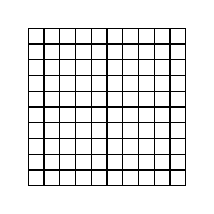
\begin{tikzpicture}[scale=1]
\foreach \x in {0,0.2,...,2}{
\draw[thin] (-2,\x) -- (0,\x);
}
\foreach \x in {-2,-1.8,...,0}{
\draw[thin] (\x,0) -- (\x,2);
}
\end{tikzpicture} &
\begin{tikzpicture}[scale=0.1]
\foreach \x in {0,2}{
\draw[thin] (-2,\x) -- (0,\x);
}
\foreach \x in {-2,0}{
\draw[thin] (\x,0) -- (\x,2);
}
\node[above] (a) at (-1,1.75) {$\frac{1}{n}$}; 
\end{tikzpicture}
\\
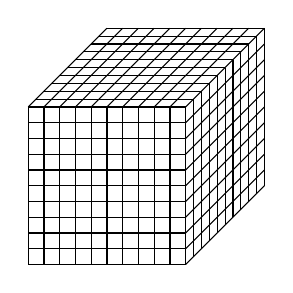
\begin{tikzpicture}[scale=1]
%front side
\foreach \x in {0,0.2,...,2}{
\draw[thin] (-2,\x) -- (0,\x);
}
\foreach \x in {-2,-1.8,...,0}{
\draw[thin] (\x,0) -- (\x,2);
}
% right side
\foreach \x in {0,0.2,...,2}{
\draw[thin] (0,\x) -- (1,\x + 1);
}
\foreach \x in {0.1,0.2,...,1}{
\draw[thin] (\x,\x) -- (\x,\x +2);
}
%top side
\foreach \x in {-2,-1.8,...,-0.2}{
\draw[thin] (\x,2) -- (\x+1,3);
}
\foreach \x in {2.1,2.2,...,3}{
\draw[thin] (\x-4,\x) -- (\x-2,\x);
}
\end{tikzpicture}
&
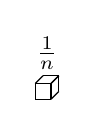
\begin{tikzpicture}[scale=.1]
%front side
\foreach \x in {0,2}{
\draw[thin] (-2,\x) -- (0,\x);
}
\foreach \x in {-2,0}{
\draw[thin] (\x,0) -- (\x,2);
}
% right side
\foreach \x in {0,2}{
\draw[thin] (0,\x) -- (1,\x + 1);
}
\foreach \x in {0,1}{
\draw[thin] (\x,\x) -- (\x,\x +2);
}
%top side
\foreach \x in {-2,-0}{
\draw[thin] (\x,2) -- (\x+1,3);
}
\foreach \x in {2,3}{
\draw[thin] (\x-4,\x) -- (\x-2,\x);
}
\node[above] (a) at (-.5,2.5) {$\frac{1}{n}$}; 
\end{tikzpicture}
\end{tabular}
\end{document}
